\documentclass[a4paper]{article}
\usepackage{newtxtext}
\usepackage[T2A]{fontenc}
\usepackage[utf8]{inputenc}
\usepackage[russian,english]{babel}
\usepackage[lmargin=30mm,rmargin=15mm]{geometry}
\usepackage[]{graphicx}

\begin{document}
\hfill
%\parbox{23mm}{dsdsd}
\parbox{75mm}{\centerКакой-то адрес\\Вторая строка\\[3mm]Адресат А.А.}
	
\begin{figure}[t]
	\centering
	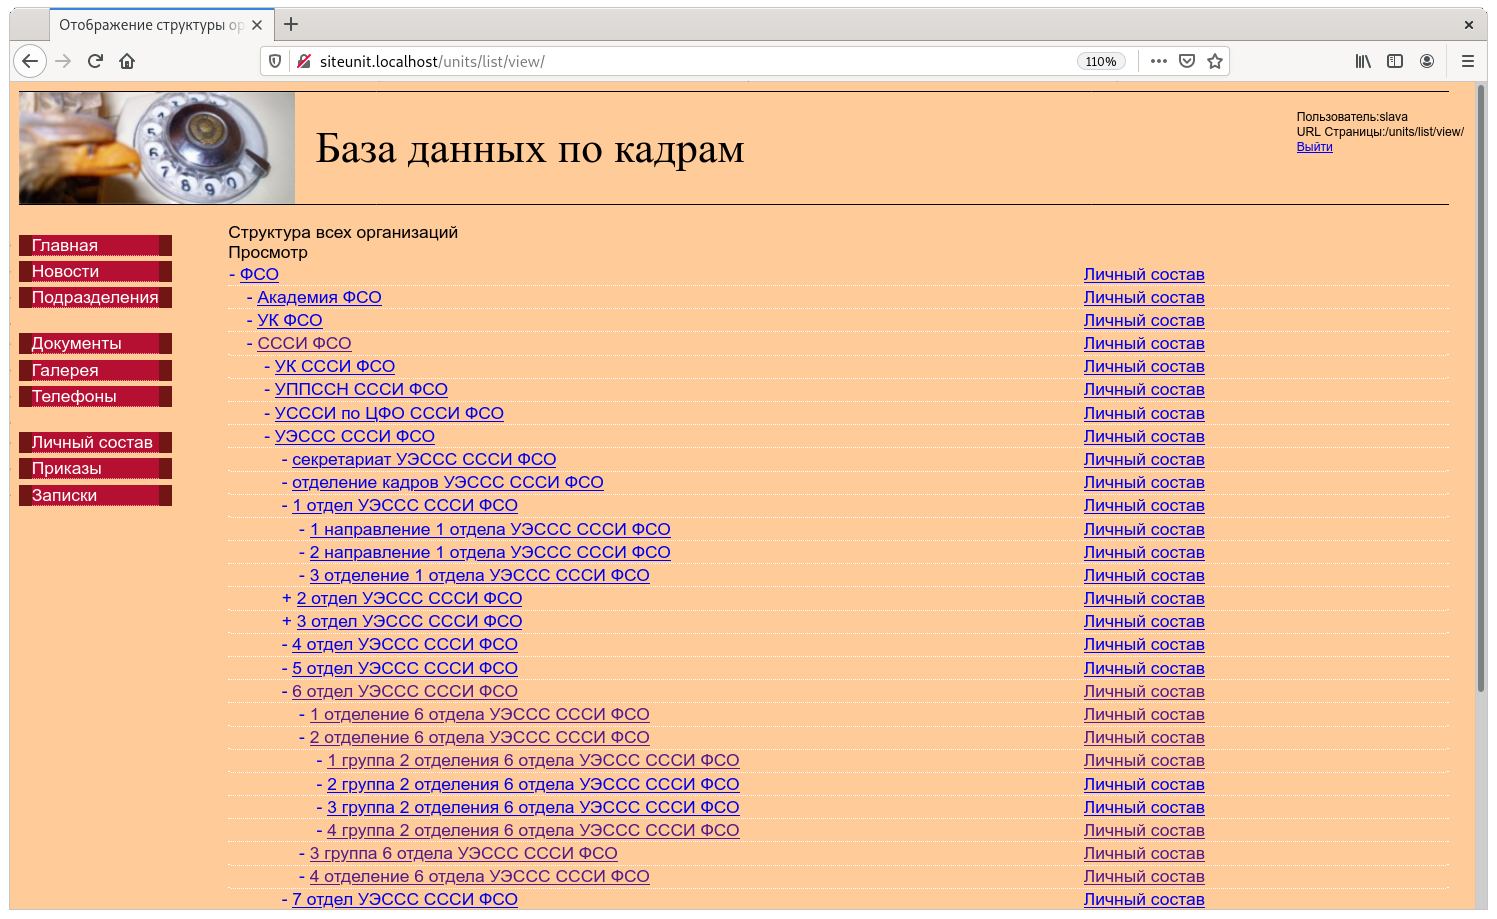
\includegraphics[width=\textwidth]{Screenshot.png}
	\caption{Снимок экрана}
	\label{fig:screenshot}
\end{figure}

%\vskip{15mm}
Это первый абзац нового документа. Здесь мы просто будем опробовать различные функции 
плагина для работы \texttt{Vim} с \LaTeX.
На рисунке \ref{fig:screenshot} что-то показано. 

proba 
$$\frac{a+b}{a-b}$$
\end{document}
